%%%%%%%%%%%%%%%%%%%%%%%%%%%%%%%%%%%%%%%%%%%%%%%%%%%%%%%%%%%%%%%%%%%%%%%%
%% Customizações do abnTeX2 (http://abnTeX2.googlecode.com)           %%
%% para a Universidade Estadual do Ceara - UECE                       %%
%%                                                                    %%
%% This work may be distributed and/or modified under the             %% 
%% conditions of the LaTeX Project Public License, either version 1.3 %%
%% of this license or (at your option) any later version.             %%
%% The latest version of this license is in                           %%
%%   http://www.latex-project.org/lppl.txt                            %%
%% and version 1.3 or later is part of all distributions of LaTeX     %%
%% version 2005/12/01 or later.                                       %%
%%                                                                    %%
%% This work has the LPPL maintenance status `maintained'.            %%
%%                                                                    %%
%% The Current Maintainer of this work is Thiago Nascimento           %%
%%                                                                    %%
%% Project available on: https://github.com/thiagodnf/uecetex2        %%
%%                                                                    %%
%% Further information about abnTeX2                                  %%
%% are available on http://abntex2.googlecode.com/                    %%
%%                                                                    %%
%%%%%%%%%%%%%%%%%%%%%%%%%%%%%%%%%%%%%%%%%%%%%%%%%%%%%%%%%%%%%%%%%%%%%%%%

%%%%%%%%%%%%%%%%%%%%%%%%%%%%%%%%%%%%%%%%%%%%%%%%%%%%%%%%%%%%%%%%%%%%%%%%
%% Customizações do abnTeX2 (http://abnTeX2.googlecode.com)           %%
%% para a Universidade Estadual do Ceara - UECE                       %%
%%                                                                    %%
%% This work may be distributed and/or modified under the             %% 
%% conditions of the LaTeX Project Public License, either version 1.3 %%
%% of this license or (at your option) any later version.             %%
%% The latest version of this license is in                           %%
%%   http://www.latex-project.org/lppl.txt                            %%
%% and version 1.3 or later is part of all distributions of LaTeX     %%
%% version 2005/12/01 or later.                                       %%
%%                                                                    %%
%% This work has the LPPL maintenance status `maintained'.            %%
%%                                                                    %%
%% The Current Maintainer of this work is Thiago Nascimento           %%
%%                                                                    %%
%% Project available on: https://github.com/thiagodnf/uecetex2        %%
%%                                                                    %%
%% Further information about abnTeX2                                  %%
%% are available on http://abntex2.googlecode.com/                    %%
%%                                                                    %%
%%%%%%%%%%%%%%%%%%%%%%%%%%%%%%%%%%%%%%%%%%%%%%%%%%%%%%%%%%%%%%%%%%%%%%%%

\documentclass[        
    a4paper,          % Tamanho da folha A4
    12pt,             % Tamanho da fonte 12pt
    chapter=TITLE,    % Todos os capitulos devem ter caixa alta
    section=TITLE,    % Todas as secoes devem ter caixa alta
    oneside,          % Usada para impressao em apenas uma face do papel
    english,          % Hifenizacoes em ingles
    spanish,          % Hifenizacoes em espanhol
    brazil            % Ultimo idioma eh o idioma padrao do documento
]{abntex2}

% Importações de pacotes
%\usepackage{rotating}				    % Rotacionar
\usepackage[utf8]{inputenc}                         % Acentuação direta
\usepackage[T1]{fontenc}                            % Codificação da fonte em 8 bits
\usepackage{graphicx}                               % Inserir figuras
\usepackage{amsfonts, amssymb, amsmath}             % Fonte e símbolos matemáticos
\usepackage{booktabs}                               % Comandos para tabelas
\usepackage{verbatim}                               % Texto é interpretado como escrito no documento
\usepackage{multirow, array}                        % Múltiplas linhas e colunas em tabelas
\usepackage{indentfirst}                            % Endenta o primeiro parágrafo de cada seção.
\usepackage{listings}                               % Utilizar codigo fonte no documento
\usepackage{xcolor}
\usepackage{microtype}                              % Para melhorias de justificação?
\usepackage[portuguese,ruled,lined]{algorithm2e}    % Escrever algoritmos
\usepackage{algorithmic}                            % Criar Algoritmos  
%\usepackage{float}                                  % Utilizado para criação de floats
\usepackage{amsgen}
\usepackage{lipsum}                                 % Usar a simulação de texto Lorem Ipsum
%\usepackage{titlesec}                               % Permite alterar os títulos do documento
\usepackage{tocloft}                                % Permite alterar a formatação do Sumário
\usepackage{etoolbox}                               % Usado para alterar a fonte da Section no Sumário
\usepackage[nogroupskip,nonumberlist,acronym]{glossaries}                % Permite fazer o glossario
\usepackage{caption}                                % Altera o comportamento da tag caption
\usepackage[alf, abnt-emphasize=bf, bibjustif, recuo=0cm, abnt-etal-cite=3, abnt-etal-list=0,abnt-etal-text=it]{abntex2cite}  % Citações padrão ABNT
%\usepackage[bottom]{footmisc}                      % Mantém as notas de rodapé sempre na mesma posição
%\usepackage{times}                                 % Usa a fonte Times
\usepackage{mathptmx}                               % Usa a fonte Times New Roman										
%\usepackage{lmodern}                               % Usa a fonte Latin Modern
%\usepackage{subfig}                                % Posicionamento de figuras
%\usepackage{scalefnt}                              % Permite redimensionar tamanho da fonte
\usepackage{color, colortbl}                       % Comandos de cores
%\usepackage{lscape}                                % Permite páginas em modo "paisagem"
%\usepackage{ae, aecompl}                           % Fontes de alta qualidade
%\usepackage{picinpar}                              % Dispor imagens em parágrafos
%\usepackage{latexsym}                              % Símbolos matemáticos
%\usepackage{upgreek}                               % Fonte letras gregas
\usepackage{appendix}                               % Gerar o apendice no final do documento
\usepackage{paracol}                                % Criar paragrafos sem identacao
\usepackage{lib/uecetex2}		                    % Biblioteca com as normas da UECE para trabalhos academicos
\usepackage{pdfpages}                               % Incluir pdf no documento
\usepackage{amsmath}                                % Usar equacoes matematicas
%\usepackage{tabu}				    % Tabelas mais flexíveis

% Organiza e gera a lista de abreviaturas, simbolos e glossario
\makeglossaries

% Gera o Indice do documento
\makeindex


%%%%%%%%%%%%%%%%%%%%%%%%%%%%%%%%%%%%%%%%%%%%%%%%%%%%%
%%          Configuracoes do ueceTeX2              %%
%%%%%%%%%%%%%%%%%%%%%%%%%%%%%%%%%%%%%%%%%%%%%%%%%%%%%

% Opcoes disponiveis

%\trabalhoacademico{tccgraduacao}
\trabalhoacademico{tccespecializacao}
%\trabalhoacademico{dissertacao}
%\trabalhoacademico{tese}

% Define se o trabalho eh uma qualificacao
% Coloque 'nao' para versao final do trabalho

\ehqualificacao{nao}

% Remove as bordas vermelhas e verdes do PDF gerado
% Coloque 'sim' pare remover

\removerbordasdohyperlink{sim} 

% Adiciona a cor Azul a todos os hyperlinks

\cordohyperlink{nao}

%%%%%%%%%%%%%%%%%%%%%%%%%%%%%%%%%%%%%%%%%%%%%%%%%%%%%
%%          Informação sobre a IES                 %%
%%%%%%%%%%%%%%%%%%%%%%%%%%%%%%%%%%%%%%%%%%%%%%%%%%%%%

\ies{Universidade Estadual do Ceará}
\iessigla{UECE}
\centro{Centro de Ciências da Saúde}
\centrosigla{Centro de Ciências da Saúde - CSS}
%%%%%%%%%%%%%%%%%%%%%%%%%%%%%%%%%%%%%%%%%%%%%%%%%%%%%
%%        Informação para TCC de Graduacao         %%
%%%%%%%%%%%%%%%%%%%%%%%%%%%%%%%%%%%%%%%%%%%%%%%%%%%%%

\graduacaoem{Enfermagem}
\habilitacao{bacharel} % Pode colocar tambem 'licenciada'

%%%%%%%%%%%%%%%%%%%%%%%%%%%%%%%%%%%%%%%%%%%%%%%%%%%%%
%%     Informação para TCC de Especializacao       %%
%%%%%%%%%%%%%%%%%%%%%%%%%%%%%%%%%%%%%%%%%%%%%%%%%%%%%

\especializacaoem{Enfermagem Obstétrica}

%%%%%%%%%%%%%%%%%%%%%%%%%%%%%%%%%%%%%%%%%%%%%%%%%%%%%
%%         Informação para Dissertacao             %%
%%%%%%%%%%%%%%%%%%%%%%%%%%%%%%%%%%%%%%%%%%%%%%%%%%%%%

\programamestrado{Programa de Pós-Graduação em Ciência da Computação}
\nomedomestrado{Mestrado Acadêmico em Ciência da Computação}
\mestreem{Ciência da Computação}
\areadeconcentracaomestrado{Ciência da Computação}

%%%%%%%%%%%%%%%%%%%%%%%%%%%%%%%%%%%%%%%%%%%%%%%%%%%%%
%%               Informação para Tese              %%
%%%%%%%%%%%%%%%%%%%%%%%%%%%%%%%%%%%%%%%%%%%%%%%%%%%%%

\programadoutorado{Programa de Pós-Graduação em Saúde Coletiva}
\nomedodoutorado{Doutorado em Saúde Coletiva}
\doutorem{Saúde Coletiva}
\areadeconcentracaodoutorado{Saúde Coletiva}

%%%%%%%%%%%%%%%%%%%%%%%%%%%%%%%%%%%%%%%%%%%%%%
%%  Informação relacionadas ao trabalho     %%
%%%%%%%%%%%%%%%%%%%%%%%%%%%%%%%%%%%%%%%%%%%%%%

\autor{Sâmela Abreu e Santiago}
\titulo{PERCEPÇÕES DO ENFERMEIRO SOBRE A VIOLÊNCIA OBSTÉTRICA NO CENTRO DE PARTO NORMAL}
\data{2019}
\local{Fortaleza -- Ceará}

% Exemplo: \dataaprovacao{01 de Janeiro de 2012}
\dataaprovacao{}

%%%%%%%%%%%%%%%%%%%%%%%%%%%%%%%%%%%%%%%%%%%%%
%%     Informação sobre o Orientador       %%
%%%%%%%%%%%%%%%%%%%%%%%%%%%%%%%%%%%%%%%%%%%%%

\orientador{Prof. Dr. Antonio Rodrigues Ferreira Júnior}
\orientadories{Universidade Estadual do Ceará – UECE}
\orientadorcentro{Centro de Ciências da Saúde - CCS}
% \orientadorfeminino{sim} % Coloque 'sim' se for do sexo feminino

%%%%%%%%%%%%%%%%%%%%%%%%%%%%%%%%%%%%%%%%%%%%%
%%      Informação sobre o Co-orientador   %%
%%%%%%%%%%%%%%%%%%%%%%%%%%%%%%%%%%%%%%%%%%%%%

% Deixe o nome do coorientador em branco para remover do documento

\coorientador{}
\coorientadories{Universidade Co-orientador - SIGLA}
\coorientadorcentro{Centro do Co-orientador - SIGLA}
\coorientadorfeminino{nao} % Coloque 'sim' se for do sexo feminino

%%%%%%%%%%%%%%%%%%%%%%%%%%%%%%%%%%%%%%%%%%%%%
%%      Informação sobre a banca           %%
%%%%%%%%%%%%%%%%%%%%%%%%%%%%%%%%%%%%%%%%%%%%%

% Atenção! Deixe o nome do membro da banca para remover da folha de aprovacao

% Exemplo de uso:
% \membrodabancadois{Prof. Dr. Fulano de Tal}
% \membrodabancadoisies{Universidade Estadual do Ceará - UECE}

\membrodabancadois{Profa. Ms. Fernanda Maria Carvalho Fontenele}
\membrodabancadoiscentro{Centro de Ciências da Saúde - CCS}
\membrodabancadoisies{Universidade Estadual do Ceará – UECE}

\membrodabancatres{Profa. Ms. Renata Borges de Vasconcelos}
\membrodabancatrescentro{Centro de Ciências da Saúde - CCS}
\membrodabancatresies{Universidade Estadual do Ceará – UECE}

\membrodabancaquatro{Prof. Ms. Alisson Salatiek Ferreira de Freitas}
\membrodabancaquatrocentro{Centro de Ciências da Saúde - CCS}
\membrodabancaquatroies{Centro Universitário Christus – Unichristus}

% \membrodabancacinco{Membro da Banca Cinco}
% \membrodabancacincocentro{Teste}
% \membrodabancacincoies{Universidade do Membro da Banca Cinco - SIGLA}
% \membrodabancaseis{Membro da Banca Seis}
% \membrodabancaseiscentro{}
% \membrodabancaseisies{Universidade do Membro da Banca Seis - SIGLA}

\begin{document}	

	% Se o seu trabalho é em ingles, descomente a linha a seguir
	%\selectlanguage{english}

	% Elementos pré-textuais
	\imprimircapa
	\imprimirfolhaderosto{}
	% \imprimirfichacatalografica{elementos-pre-textuais/ficha-catalografica}
	%\imprimirerrata{elementos-pre-textuais/errata}
	\imprimirfolhadeaprovacao
	% \imprimirdedicatoria{elementos-pre-textuais/dedicatoria}
	\imprimiragradecimentos{elementos-pre-textuais/agradecimentos}
	% \imprimirepigrafe{elementos-pre-textuais/epigrafe}
	\imprimirresumo{elementos-pre-textuais/resumo}
	\imprimirabstract{elementos-pre-textuais/abstract}
	%\imprimirlistadeilustracoes
	%\imprimirlistadetabelas
	%\imprimirlistadequadros
	%\imprimirlistadealgoritmos
	%\imprimirlistadecodigosfonte
	\imprimirlistadeabreviaturasesiglas	
	%\imprimirlistadesimbolos{elementos-pre-textuais/lista-de-simbolos}   
	\imprimirsumario
	
	%Elementos textuais
	\textual
	\chapter{Introdução}
\label{cap:introducao}

O \acrlong{SUS} (\acrshort{SUS}) é composto de níveis de atenção (primário, secundário e terciário) em que geralmente a Atenção Básica deve ser o contato preferencial dos usuários, porta de entrada e centro de comunicação com toda a Rede de Atenção à Saúde \citeonline{ministerio2012politica}.

O enfermeiro está presente em todos os  níveis de atenção desenvolvendo atividades tanto assistenciais quanto gerenciais. Mesmo com a sua presença em ambientes tão diversos é na \acrlong{AB} (\acrshort{AB}) que suas habilidades tem potencial para se desenvolver com maior autonomia. 

Em um estudo de \citeonline{kalinowski2013autonomia}, os enfermeiros perceberam que tinham autonomia profissional quando surgiam situações com a possibilidade de tomar decisões no serviço de saúde e também no seu processo de trabalho, utilizando dispositivos indispensáveis como competência, responsabilidade, respeito e reconhecimento na equipe interdisciplinar.

Essa autonomia decorre não apenas de uma postura profissional, o saber-ser do enfermeiro, mas também da própria dinâmica da \acrshort{AB}, que enfatiza uma assistência multidisciplinar ao paciente e às comunidades. 

No mesmo estudo, comprovou-se que a enfermeira exerce no seu campo de trabalho diferentes atividades, cabendo à ela, reorganizar tanto o seu processo de trabalho, quanto  o da sua equipe, criando assim, maior visibilidade da sua prática. 

Este profissional é muitas vezes o articulador da equipe de saúde na AB, pois com suas competências gerenciais, tem no trabalho em equipe um caminho para a comunicação e contato entre os diferentes profissionais. Para \citeonline{rocha2013avaliaccao}, graças às atribuições do enfermeiro na \acrlong{ESF} (\acrshort{ESF}), este vem assumindo cada vez mais o papel de gerente das unidades. Isto exige dele um olhar mais amplo sobre o trabalho, despertando o reconhecimento dos outros profissionais como articulador, facilitador e mediador de muitas ações. 

A \acrshort{ESF} é uma estratégia que visa reorganizar a \acrshort{AB} no país de acordo com os preceitos do \acrshort{SUS}. Ela tem caráter de expansão, qualificação e consolidação da \acrshort{AB}, pois favorece reorientação do processo de trabalho com potencial de aprofundar princípios, diretrizes e fundamentos da \acrshort{AB}, ampliando sua resolutividade e impacto na situação de saúde das pessoas e coletividades, além de proporcionar uma importante relação de custo-efetividade \cite{ministerio2012politica}.

Para isso ela apresenta equipes multidisciplinares, que minimamente são formadas por por um médico generalista ou especialista em Saúde da Família, um enfermeiro generalista ou especialista em Saúde da Família, auxiliar ou técnico de enfermagem e agentes comunitários de saúde, podendo-se a esta acrescentar os profissionais de saúde bucal \cite{ministerio2012politica}.

Considerando-se as diferentes realidades de cada local, as diversas Unidades Básicas de Saúde (\acrshort{UBS}) que compõe a \acrshort{AB} precisam de uma articulação entre seus profissionais e os demais componentes do sistema de saúde, além de articulação também com as comunidades na qual estão inseridas de forma a oferecer assistência tendo como base os princípios da universalidade, da acessibilidade, do vínculo, da continuidade do cuidado, da integralidade da atenção, da responsabilização, da humanização, da equidade e da participação social e um processo de comunicação que vá contribuindo para autonomização e protagonismo de sujeitos nos processos de tomada de decisão.

Assim, a comunicação é uma dos principais componentes para o funcionamento de qualquer grupo. É a competência interpessoal capaz de decodificar as diversas formas de expressão humana capaz de ampliar as relações num dado território \cite{rocha2013avaliaccao}.

Neste processo de comunicação, tem-se a formação de redes sociais. O conceito de Redes Sociais não é novo e nem restrito. Para \citeonline{marteleto2010redes}, é um conceito presente atualmente em diversos espaços e parece servir a dois propósitos: caracterizar o espaço em que a comunicação ocorre no mundo globalizado de hoje onde se tem a produção de formas diferentes de ações coletivas, expressão de identidades, conhecimentos informação e cultura; e para apontar as mudanças no modo de se comunicar e passar adiante a informação, ou seja, modos de compartilhá-la.

Assim sendo, \citeonline{marteleto2010redes} também coloca que as informações e as redes sociais são dois conceitos que se encontram e que permeiam diferentes domínios de conhecimento, mídias, campos sociais ou comunidades profissionais. A troca de informações, seu uso e apropriação vão depender de como as pessoas e grupos envolvidos no processo de comunicação se associam.

Uma proposta para a análise dessas relações que se formam está na \acrlong{ARS} (\acrshort{ARS}) que é uma ferramenta que nos permite conhecer as interações entre qualquer classe de indivíduos, partindo preferencialmente de dados qualitativos do que quantitativos \cite{alejandro2005manual}.

Na saúde, a \acrlong{ARS} tem como foco a compreensão das relações entre os atores, ou seja, das relações entre os profissionais de diferentes categorias que participam do processo de comunicação, durante o cuidado prestado aos pacientes \cite{antonio2013}.
 
Consiste em uma ramo do campo de estudo das relações interorganizacionais que pode monitorar como ocorrem as trocas presentes na produção do serviço de saúde, observando de que forma a localização dos atores envolvidos se relaciona com poder e influência \cite{bittencourt2009rede}.

Nesse contexto, os pacientes das várias linhas de cuidado são beneficiados com o bom funcionamento da comunicação, cooperação e do vínculo dos profissionais da unidade na qual são assistidos e da unidade com os outros serviços de saúde disponíveis. 

Segundo \citeonline{cecilio2003integralidade}, a concepção de linha de cuidado ilustra a produção da saúde de forma sistêmica, partindo das redes macro e microinstitucionais, com processos dinâmicos, onde se tem a imagem da linha de produção direcionada ao fluxo de assistência àquele que dela irá se beneficiar de acordo com suas necessidades.

A linha de cuidado pode ser abordada nas perspectivas de macro e micropolítica. Na micropolítica, tem-se o encontro entre o usuário e o profissional e nela, torna-se essencial que a assistência passe de procedimentos fragmentados a ações de responsabilização, vinculação e cuidado, possibilitando assim projetos terapêuticos singularizados \cite{malta2010percurso}.

Quanto a macropolítica, tem-se as relações entre os gestores e profissionais envolvidos no cuidado, fomentando corresponsabilização de forma a garantir apoio para as ações de cuidado \cite{malta2010percurso}.

Dentre os que mais buscam o atendimento a nível primário, encontramos os pacientes com \acrlong{HAS} (\acrshort{HAS}) e \acrlong{DM} (\acrshort{DM}). Estes pacientes muitas vezes requerem um atendimento diferenciado envolvendo uma diversidade de ações de cuidado que são implementadas por diferentes profissionais. Isto se deve ao aspecto crônico dessas patologias e aos fatores e determinações  a elas associados. 

Existe também a possibilidade do desenvolvimento de comorbidades associadas ao estado sistêmico em que o indivíduo se encontra, tudo isso dependendo do estilo de vida e seus modos de compreender a produção da saúde desses pacientes, envolvendo ainda seu contexto familiar e social. 

Por exemplo, em um estudo desenvolvido com idosos hipertensos de um município do Paraná, \citeonline{ferrari2014motivos}, identificaram que as principais queixas que levavam esses pacientes a buscarem os serviços da \acrshort{UBS} eram relacionados a doenças endócrinas, nutricionais e metabólicas. Consistiam em problemas como excesso de peso, elevação de níveis glicêmicos e hipercolesterolemia. Demandas como essas podem envolver toda a equipe em um cuidado que requer diversas abordagens profissionais. 

Este contexto colabora para tornar o acompanhamento da \acrshort{HAS} e \acrshort{DM} na atenção primária um fator que pode evitar o surgimento e progressão de complicações. Isto faz com que se reduzam as internações hospitalares e mortalidade relacionada a esses agravos \cite{da2012associaccao}.

A \acrshort{AB} para esses pacientes funciona então não só como porta de entrada, mas como importante território de matriciamento para acompanhamento e suporte à nova realidade a que esses pacientes devem se adaptar. Além disso, cuidados especializados devem ser providenciados através do sistema de referência, encaminhando o paciente a outros serviços dentro do sistema de saúde. 

Uma vez que o enfermeiro se localiza em uma posição primordial para articular ações que promovam o acesso aos serviços de saúde e a continuidade do cuidado, contemplando assim a integralidade da assistência, através da comunicação e da ativação de sua própria rede social ou interpessoal, questiona-se: como se configura a Rede Social para a linha de cuidado a pacientes hipertensos e diabéticos de uma enfermeira da \acrshort{ESF} de um município de pequeno porte?

\section{Justificativa}
A escolha pelo tema teve origem com a vivência como acadêmica da disciplina Internato I durante o módulo de Atenção Básica na \acrshort{ESF} em Pacoti-Ce. Como este sendo um município de pequeno porte, foi-me possível observar a rede de assistência com mais detalhes e percebi que em diversas situações a enfermeira da equipe intermediava ações de cuidado e assistência dos profissionais da unidade e com as demais instituições da rede municipal de saúde, além de acionar a participação de indivíduos da comunidade que facilitavam o acesso a variados equipamentos sociais que eram utilizados para o desenvolvimento de atividades de educação em saúde na comunidade. 

Percebi também a constante busca pela população com \acrshort{HAS} e \acrshort{DM}, que prioritariamente buscava a consulta médica devido a prescrição de algumas medicações, mas que quando passavam pela consulta de enfermagem, relatavam outras demandas. Em muitas dessas situações, a enfermeira recorria aos próprios contatos no hospital municipal, na Secretaria de Saúde, além do contato direto com os Agentes Comunitários de Saúde (\acrshort{ACS}) e os demais profissionais da unidade. Essas situações geralmente se relacionavam a falta de acesso a um serviço ou a demora na resolução de uma demanda. 

Contou também para a escolha do tema o interesse em novas metodologias para análises no campo da Saúde Coletiva, sobretudo ligadas ao processo de trabalho do enfermeiro. Essas discussões foram suscitadas durante algumas reuniões do grupo de pesquisa Políticas, Saberes e Práticas em Enfermagem e Saúde Coletiva da \acrlong{UECE} (\acrshort{UECE}).  

\section{Relevância}
Baseado  no exposto é relevante mapear esta forma de enfrentamento de múltiplas situações que incidem sobre o processo de trabalho do enfermeiro e assim compreender melhor os elementos que permitem a este profissional configurar, participar e/ou liderar, explicita ou tacitamente as redes sociais visando responder às demandas e necessidades cotidianas dos usuários hipertensos e diabéticos. 

Além disso, o presente estudo serve como passo inicial na investigação de como contribuir para a reorganização do processo de trabalho da equipe multidisciplinar da unidade  básica com os outros serviços da rede de forma mais  efetiva, solidária e cooperativa, facilitando o acesso e o cuidado integral dos pacientes dessa linha de cuidado.
	\section{Objetivos}
\label{sec:objetivos}

\subsection{Objetivo Geral}
\label{sec:objetivo-geral}

Conhecer o papel do enfermeiro na articulação das Redes Sociais de Apoio dos usuários no âmbito da Atenção Básica de acordo com a literatura.

\subsection{Objetivos Específicos}
\label{sec:objetivos-especificos}

\begin{alineas}
	\item Explorar os conceitos de Rede Social, Apoio Social e Rede Social de Apoio de acordo com a literatura;
	\item Conhecer a participação do enfermeiro nessas redes sociais de apoio e quais as implicações dela no cuidado integral à saúde dos indivíduos e das comunidades.
\end{alineas}
	\chapter{Revisão de Literatura}
\label{sec:revisao}

\section{A Sífilis na Gestação: um problema simples e longe de resolução}
A sífilis, por ser quase que facilmente transmitida pelo contato sexual, é considerada uma infecção sexualmente transmissível, pandêmica que inicia seu ciclo por meio de cancros, evoluindo posteriormente para sua forma crônica. Pode afetar diversos sistemas do organismo e sem tratamento adequado, pode levar a óbito. Em alguns casos ela pode infectar o feto por transmissão vertical via transplacentária, ocasionando a sífilis congênita. \cite{silva2015feelings}

É também um importante problema de saúde pública, pois além de seu potencial infectocontagioso, ela pode debilitar de modo grave o organismo e quando não tratada, aumenta o risco para infecção do HIV por meio de suas lesões que servem como porta de entrada. \cite{manual2016sifilis}

Sem tratamento, a sífilis progride apresentando três fases sintomáticas, permeadas por períodos assintomáticos (fases latentes). Determinar o estágio em que ela se apresenta é importante para o método diagnóstico. Entretanto é uma doença difícil de diagnosticar, justamente por ter períodos sem manifestações de sintomas, além de período de incubação variável. \cite{manual2016sifilis}

A sífilis primária apresenta úlcera única, endurecida e não dolorosa  na região genital, o cancro duro. Essa lesão pode desaparecer naturalmente, mesmo sem tratamento. Já a sífilis secundária, se apresenta entre seis e oito semanas após a primeira lesão podendo manifestar lesões cutâneas e nas mucosas, sendo comum as roséolas. O indivíduo pode ou não ter febre, mal-estar, fraqueza muscular e cefaléia. Aqui as lesões são mais visíveis, mas também desaparecem. A sífilis terciária só aparece de 3 a 12 anos depois do contágio, apresenta lesões neurológicas e complicações mais sérias: problemas ósseos e cardiovasculares. Os períodos de latência não apresentam sintomas e são diferenciados em recente (menos de um ano) e tardia (mais de um ano). Nesse caso a doença só é detectada por meio de testes sorológicos. \cite{manual2016sifilis}

Quanto às gestantes, se não tratadas adequadamente, podem ocasionar a transmissão vertical, gerando a sífilis congênita. Essa transmissão se torna mais provável quanto mais recente for a infecção. 

No período gestacional o diagnóstico e tratamento ocorrem durante as consultas de  pré-natal. Todas as gestantes e suas parcerias sexuais precisam ser investigadas  e também informadas sobre as formas de contágio e riscos para a gestação e o bebê. Pelo protocolo do Ministério da Saúde, o uso de testes-rápidos servem como triagem para gestantes e seus parceiros. Embora essa seja uma intervenção eficaz,  depende de muitos fatores para ser efetiva. Já o VDRL é solicitado logo na primeira consulta de pré-natal, de preferência ainda no primeiro trimestre gestacional. O teste rápido também é realizado no início do terceiro trimestre e no momento do parto. Além disso, deve ser realizado também em casos de abortamento. \cite{brasil2015protocolo}

Para um diagnóstico mais completo incluindo o estadiamento da infecção, usam-se testes treponêmicos e o VDRL, pois ambos são complementares, uma vez que juntos, diminuem o erro por conta de falsos positivos e negativos. Os testes treponêmicos identificam anticorpos específicos para o Treponema pallidum, agente etiológico da sífilis, sendo usado na triagem ou confirmação de resultado. \cite{sao2016guia}

Toda gestante diagnosticada com sífilis deve iniciar o tratamento imediatamente. A única forma de tratamento efetivo é o uso da penicilina G benzatina. O parceiro também é procurado para teste rápido e posterior tratamento. Em caso de sensibilização da gestante à penicilina, inicia-se tentativa de dessensibilização em serviços de saúde especializados. Caso seja impossível o processo, o tratamento é feito com ceftriaxona, entretanto é considerado um tratamento inadequado e neste caso, o recém-nascido será avaliado clínica e laboratorialmente. \cite{sao2016guia}

O tratamento na gestante é considerado adequado quando: é completo, documentado e adequado ao estágio da doença, sendo realizado com penicilina G benzatina; o parceiro também é tratado; a gestante apresenta queda em suas titulações para os testes sorológicos não-treponêmicos, ou estáveis se os títulos forem menores ou iguais que 1:4. \cite{sao2016guia}

É possível observar através de manuais frequentemente elaborados que os processos para rastreamento, diagnóstico e tratamento da gestante estão bem estabelecidos e institucionalizados transversalmente pelo Ministério da Saúde por meio de programas, estratégias e políticas. Mesmo assim, a sífilis na gestação e também a congênita, continuam a ser um problema longe de ser solucionado, pois dependem de diversos fatores ligados não apenas a assistência e a gestão, como também a cultura, nível socioeconômico e outros. 

Para \cite{cad2013} a sífilis em gestantes se relaciona ao baixo nível socioeconômico. Mesmo não se restringindo à população menos favorecida, os resultados de seu estudo indicam que pouca escolaridade e baixa renda podem ser sinais importantes de acesso limitado aos serviços de  saúde.

Até mesmo no que se refere às notificações de casos, surgem falhas nesse processo, o que leva a um mal direcionamento das políticas públicas para sua prevenção e controle. 

Para \cite{domingues2016incidencia}, a quantidade de casos notificados depende da capacidade de intervenção direcionada a redução da transmissão vertical; diagnóstico e tratamento bem executados tanto das gestantes quanto de seus parceiros e da notificação correta, pois números baixos de casos de sífilis não garantem que a assistência está sendo eficiente no controle da doença, pois pode estar havendo subnotificação. Ao mesmo tempo, um alto número de casos indica falhas na assistência.

O controle da sífilis e de de outras IST no Brasil precisa ser um processo dinâmico, sendo renovado constantemente, necessitando de protagonismo por parte dos trabalhadores da saúde, além das responsabilidades de cada órgão que compõe o SUS. É fundamental a existência de saberes e práticas de gestão para que as políticas possam ser estruturadas e executadas de acordo com os princípios do SUS. \cite{brasil2015protocolo}


	\chapter{Metodologia}
\label{chap:metodologia}

Neste trabalho, realizou-se uma revisão integrativa de artigos relacionados às ações tomadas por enfermeiros nas consultas a gestante com sífilis gestacional de modo a aumentar a adesão ao tratamento.

As revisões são métodos de pesquisa que servem para fornecer conhecimentos sobre um problema de pesquisa específico, sendo esse conhecimento transformado em prática posteriormente. No que se refere a revisão integrativa, esta é usada para sintetizar informações obtidas a respeito de um assunto de maneira sistemática, ordenada e abrangente. Sendo abrangente ela pode ter diferentes fins: definir conceitos, rever teorias ou analisar métodos de estudos sobre um tema específico. \cite{mendes2005revisao}

Seguiram-se os seguintes passos nesta revisão: identificação do problema com delineamento claro do propósito do estudo, pesquisa nas bases de dados por literatura pertinente utilizando descritores, formulação da base de dados e uso dos critérios de inclusão e exclusão para seleção dos artigos e avaliação dos achados com posterior apresentação dos resultados. \cite[p. 04]{teixeira2014integrative}.

Os dados foram levantados por meio de pesquisa pareada e independente no site da \acrshort{BVS} (\acrlong{BVS}), em janeiro de 2019 utilizando-se os descritores presentes no \acrshort{DeCS} (\acrlong{DeCS}): sífilis, enfermagem e pré-natal, colocando-se o booleando AND entre os termos. Foram encontradas 30 publicações. Após a aplicação dos critérios de inclusão e exclusão, selecionaram-se os artigos que compuseram a amostra do estudo.

Optou-se como critérios de inclusão: estudos em língua portuguesa, inglesa e espanhola; publicados de 2008 a 2019; realizados no Brasil, disponíveis online e na íntegra que abordavam as ações tomadas por enfermeiros no pré-natal a gestantes com sífilis para a adesão de tratamento de sífilis gestacional. 

Os critérios de exclusão adotados foram: publicações que não fossem artigos científicos, outras revisões ou reflexões, estudos que não foram desenvolvidos no Brasil, estudos repetidos ou que não respondessem o objetivo desta pesquisa. 

Das 30 publicações iniciais, 21 estavam disponibilizadas integralmente. Entretanto,  apenas 14 eram artigos. As outras publicações eram 06 teses e 01 recurso de educação aberto. Foram analisados os 14 artigos, dos quais 06 foram escolhidos com base nos critérios para compor a amostra do estudo. Os excluídos tratavam-se de 02 revisões, 01 artigo de reflexão, 01 artigo repetido, 01 não disponível online, 01 anais de congresso e 01 estudo não realizado no Brasil. 

Quanto às bases de dados, os artigos que compuseram a amostra estavam disponíveis nas bases de dados \acrlong{BDENF} (\acrshort{BDENF}) - Enfermagem (5) e \acrlong{LILACS} (\acrshort{LILACS}) (1).

Depois da leitura e fichamento dos trabalhos pesquisados, realizou-se à análise descritiva e de conteúdo dos mesmos, contribuindo para a reflexão sobre o tema abordado neste trabalho. 

% Para atingir os objetivos desta pesquisa, foi escolhido o método de revisão integrativa que ``combina dados da literatura teórica e empírica, além de incorporar um vasto leque de propósitos, como: definição de conceitos, revisão de teorias e evidências, análise de problemas metodológicos.'' \cite[p. 04]{teixeira2014integrative}.

% Em meio a uma variedade de formas de se realizar uma revisão integrativa, alguns aspectos devem ser respeitados de forma a garantir um trabalho com rigor metodológico. Assim, essa revisão será constituída dos seguintes passos: identificação do problema com claro delineamento do propósito do estudo, busca nas bases de dados por literatura pertinente utilizando descritores ou palavras-chave, formulação da base de dados e uso dos critérios de inclusão e exclusão para seleção dos artigos e avaliação dos achados com posterior apresentação dos resultados. \cite[p. 04]{teixeira2014integrative}.

% Os dados serão levantados nas bases de dados \acrlong{MEDLINE} (\acrshort{MEDLINE}), \acrlong{LILACS} (\acrshort{LILACS}) e \acrlong{SciELO} (\acrshort{SciELO}), consideradas as principais da área da saúde brasileira. 

% Visando garantir o rigor metodológico, a busca dos artigos será feita pelos dois revisores concomitantemente e serão utilizados os termos considerados descritores no \acrlong{DeCS} (\acrshort{DeCS}): Rede Social, Apoio Social, Cuidado de Enfermagem e Enfermagem da Família. 

% Como critérios de inclusão optou-se por: estudos em língua portuguesa, inglesa e espanhola; publicados de 2005 a 2015; que abordem os conceitos de redes sociais e que tragam o enfermeiro envolvido nesse processo de formação; que sejam de livre acesso, disponíveis online e na íntegra, e que foram produzidos no Brasil, pois é a realidade que se quer abordar. 

% Como critérios de exclusão tem-se: estudos desenvolvidos em outros países, guidelines, artigos de revisão, protocolos, estudos que aparecerem em mais de uma base de dados, que estejam fora do recorte de tempo e que não respondam aos objetivos da pesquisa. 

% Após a coleta do material ambos os revisores, separadamente, darão início a suas leituras e executarão a extração dos dados que respondam aos objetivos. Os achados serão confrontados, verificando-se onde os estudos convergem e divergem, e posteriormente, eles serão organizados analisados e categorizados tematicamente de acordo com os temas que mais surgirem.  

	\chapter{Resultados}
\label{chap:resultados}

Após a análise de forma criteriosa e detalhada dos estudos selecionados, identificando abordagens, objetos de estudo e relação com a temática, apenas os 06 estudos foram analisados. A seguir, tem-se a caracterização dos mesmos, evidenciando-se a base em que se encontravam, os autores do estudo, a cidade ou estado brasileiro em que foram desenvolvidos, a amostra, o interesse do estudo (objetivos), o tipo de estudo, local de coleta de dados, as ações desenvolvidas no pré-natal e por fim, estratégia que facilitasse a adesão ao tratamento.

\section{Assistência Pré-natal no contexto da estratégia de saúde da família \cite{dos2010assistencia}}

\begin{description}
\item \textbf{Base de dados}: BDENF-Enfermagem
\item \textbf{Autores}: Hélcia Carla dos Santos Pitombeira, Liana Mara Rocha Teles, Jamile de Souza Pacheco Paiva, Maysa Oliveira Rolim, Lydia Vieira Freitas, Ana Kelve de Castro Damasceno.
\item \textbf{Cidade/Estado/ País}: São Gonçalo do Amarante/Ceará/Brasil
\item \textbf{Amostra}: 632
\item \textbf{Interesse do Estudo}: Estudar o acompanhamento pré-natal oferecido no município de São Gonçalo do Amarante com base nas informações do SIAB, SISPRENATAL, SINASC, SINANNET e SIM.
\item \textbf{Tipo de Estudo}: Estudo descritivo, com abordagem quantitativa
\item \textbf{Local do Estudo}: SIAB, SISPRENATAL, SINASC, SINANNET e SIM
\item \textbf{Ações na consulta de pré-natal}: Exames VDRL
\item \textbf{Estratégia para adesão}: Busca ativa (realizada pelo ACS)
\end{description}

\section{Assistência pré-natal a gestante com diagnóstico de sífilis \cite{suto2016assistencia}}

\begin{description}
\item \textbf{Base de dados}: BDENF-Enfermagem
\item \textbf{Autores}: Cleuma Sueli Santos Suto, Débora Lima da Silva, Eliana do Sacramento de Almeida, Laura Emmanuela Lima Costa, Taiana Jambeiro Evangelista.
\item \textbf{Cidade/Estado/ País}: Jacobina/Bahia/Brasil
\item \textbf{Amostra}: 667 (SINAN e SisPreNatal) e 6 no estudo de campo (3 enfermeiras e 3 gestantes)
\item \textbf{Interesse do Estudo}: Investigar qual tem sido a assistência prestada às gestantes com sífilis na Atenção Básica.
\item \textbf{Tipo de Estudo}: Estudo transversal e exploratório
\item \textbf{Local do Estudo}: SINAN, SisPreNatal e nas unidades de Saúde da Família e residência das gestantes do município de Jacobina-Bahia.
\item \textbf{Ações na consulta de pré-natal}: Prescrição de penicilina G benzatina
\item \textbf{Estratégia para adesão}: Atividades educativas sobre sífilis na UBS
\end{description}

\section{Monitoramento das ações pró-redução da transmissão vertical da sífilis na rede pública do Distrito Federal \cite{tavares2012monitoramento}}

\begin{description}
\item \textbf{Base de dados}: BDENF-Enfermagem
\item \textbf{Autores}:     Leonor Henriette de Lannoy Coimbra Tavares, Onã Silva, Leidijany Costa Paz, Luís Antônio Bueno Lopes, Maria Liz Cunha de Oliveira, Maria Marta Lopes Macedo, Sônia Geraldes
\item \textbf{Cidade/Estado/ País}: Distrito Federal/Brasil
\item \textbf{Amostra}: 3.726
\item \textbf{Interesse do Estudo}: Analisar o perfil epidemiológico e a cobertura de realização do VDRL durante a gestação e o parto, em gestantes e parturientes atendidas na rede pública de saúde do Distrito Federal.
\item \textbf{Tipo de Estudo}: Epidemiológico
\item \textbf{Local do Estudo}: Hospital Regional da Asa Sul, Hospital Regional da Asa Norte, Hospital Regional da Ceilândia, Hospital Regional de Brazilândia, Hospital Regional de Taguatinga, Hospital Regional de Sobradinho, Hospital Regional de Planaltina, Hospital Regional de Samambaia, Hospital Regional do Gama,  Hospital Regional do Paranoá e Hospital Universitário de Brasília.
\item \textbf{Ações na consulta de pré-natal}: Preenchimento do cartão das gestantes incompleto, poucas gestantes apresentavam 3 VDRL no pré-natal. 
\item \textbf{Estratégia para adesão}: Não há
\end{description}

\section{Avaliação da assistência pré-natal em município do Sul do Brasil \cite{segatto2015evaluation}}

\begin{description}
\item \textbf{Base de dados}: BDENF-Enfermagem
\item \textbf{Autor}: Marília Judith Segatto, Suzinara Beatriz Soares de Lima, Marciane Kessler, Thais Dresch Eberhardt, Rhea Silvia de Avila Soares, Lidiana Batista Teixeira Dutra Silveira
\item \textbf{Cidade/Estado/ País}: Município de Segredo-Rio Grande do Sul do Brasil
\item \textbf{Amostra}: 80 gestantes.
\item \textbf{Interesse do Estudo}: Verificar a efetividade da assistência pré-natal por meio de indicadores de processo de um município da região Sul do Brasil.
\item \textbf{Tipo de Estudo}: Estudo descritivo, com delineamento documental, utilizando indicadores de processo da assistência pré-natal do período de janeiro a dezembro de 2011, por meio do Sistema de Acompanhamento do Programa de Humanização no Pré-Natal e Nascimento.
\item \textbf{Local do Estudo}: SISPRENATAL implantado no setor de Epidemiologia da Secretaria Municipal de Saúde.
\item \textbf{Ações na consulta de pré-natal}: VDRL, consultas, preenchimento inadequado do cartão da gestante
\item \textbf{Estratégia para adesão}: Não há
\end{description}

\section{Sífilis congênita no Ceará: análise epidemiológica de uma década \cite{da2013sifilis}}

\begin{description}
\item \textbf{Base de dados}: LILACS
\item \textbf{Autor}: Camila Chaves da Costa, Lydia Vieira Freitas, Deise Maria do Nascimento Sousa, Lara Leite de Oliveira, Ana Carolina Maria Araújo Chagas, Marcos Venícios de Oliveira Lopes, Ana Kelve de Castro Damasceno
\item \textbf{Cidade/Estado/ País}: Ceará/Brasil
\item \textbf{Amostra}: 10.000 nascidos vivos. 2.930 casos de sífilis congênita.
\item \textbf{Interesse do Estudo}: avaliar a taxa de notificação de sífilis congênita no estado do Ceará nos anos de 2000 a 2009 de acordo com a base de dados do Sistema Nacional de Agravos de Notificação- SINAN, descrever o perfil epidemiológico das gestantes cujos recém-nascidos tiveram sífilis congênita; verificar a realização do pré-natal e tratamento das gestantes cujos recém-nascidos tiveram sífilis congênita e a realização do tratamento de seus parceiros.
\item \textbf{Tipo de Estudo}: Estudo do tipo transversal e documental, com abordagem quantitativa.
\item \textbf{Local do Estudo}: Estudo documental, realizado em julho de 2010 a partir do banco de dados disponível no Núcleo de Informação e Análise em Saúde (NUIAS) da Secretaria de Saúde do Estado do Ceará (SESA- CE)
\item \textbf{Ações na consulta de pré-natal}: consultas realizadas de forma inadequada
\item \textbf{Estratégia para adesão}: Não há.
\end{description}

\section{Sífilis Na Gestação: Perspectivas e Condutas do Enfermeiro \cite{nunes2017sifilis}}

\begin{description}
\item \textbf{Base de dados}: BDENF-Enfermagem
\item \textbf{Autor}: Jacqueline Targino Nunes, Ana Caroline Viana Marinho, Rejane Marie Barbosa Davim, Gabriela Gonçalo de Oliveira Silva, Rayane Saraiva Felix, Milva Maria Figueiredo de Martino
\item \textbf{Cidade/Estado/ País}: Natal/Rio Grande do Norte/Brasil
\item \textbf{Amostra}: 4 enfermeiros 
\item \textbf{Interesse do Estudo}: Discutir as ações do enfermeiro na atenção pré-natal a gestantes com sífilis e identificar dificuldades encontradas pelos profissionais na adesão ao tratamento das gestantes e parceiros.
\item \textbf{Tipo de Estudo}: Estudo qualitativo, tipo descritivo-exploratório.
\item \textbf{Local do Estudo}: Unidade Mista Felipe Camarão
\item \textbf{Ações na consulta de pré-natal}: Interrogar sobre o estado da gestante, avaliar a efetividade e adesão ao tratamento dela e do parceiro. Orientar quanto à importância do tratamento, riscos para a sífilis congênita. Encaminhamento da gestante para tratamento medicamentoso. Identificar gestantes com sinal de alarme e/ou identificadas como de alto risco e encaminhá-las para consulta médica.
\item \textbf{Estratégia para adesão}: Informação a respeito do direito do teste mensalmente, solicitação mensal do VDRL. Acolher o paciente de forma que ela/ele se sinta segura(o) dando as devidas orientações. Desenvolver atividades educativas, individuais e em grupos. Orientar gestantes e a equipe quanto aos fatores de risco e à vulnerabilidade.
\end{description}

\chapter{Discussão}
\label{chap:discussao}

Observa-se que os estudos trazem a sífilis gestacional sob o enfoque de diferentes tipos de estudos. Entretanto, a abordagem quantitativa foi a mais adotada. A maioria dos trabalhos adotou como sua fonte de dados os sistemas de informação em especial o \acrshort{SINAN} (2) e o \acrshort{SISPRENATAL} (\acrlong{SISPRENATAL}) (3). Em se tratando dos estudos de abordagem qualitativa, houve um do tipo descritivo-exploratório que fez uso de entrevistas e análise de conteúdo.

Neste trabalho, optou-se por realizar uma revisão integrativa para entender melhor como se dá o atendimento à gestante com sífilis no pré-natal. Deu-se especial atenção a trabalhos que abordam ações da enfermagem no combate a essa enfermidade por meio de estratégias para a adesão das pacientes e seus parceiros ao tratamento, melhorando assim os indicadores referentes a sífilis congênita e a qualidade da assistência como um todo dentro do que se preconiza o \acrlong{PHPN} (\acrshort{PHPN}).

Os estudos tiveram como interesses principais identificar o perfil epidemiológico das gestantes com sífilis, avaliar com base nos dados de sistemas de informação se a assistência no pré-natal a pacientes com sífilis estava sendo realizada de modo adequado e com cobertura suficiente, apontar os problemas relacionados ao pré-natal de gestantes com sífilis, apontar quais atividades da consulta do enfermeiro e mesmo se houve subnotificação de casos de sífilis. 

O perfil identificado nos trabalhos revela que a maior parte das gestantes que realizaram as consultas de pré-natal eram pessoas socialmente vulneráveis com baixo nível de escolaridade, baixo nível socioeconômico e pouca idade. Existe ainda um estudo que aponta a questão racial como fator excludente ao acesso dos exames de prevenção e tratamento. \cite{dos2010assistencia,suto2016assistencia,tavares2012monitoramento,da2013sifilis}

Fica clara a importância do Estado na promoção da saúde através de iniciativas educacionais e comprometimento dos órgãos de gestão (secretarias de saúde) a estruturarem os serviços de saúde de modo a permitir a implementação dessas ações e atingir o público mais carente. Uma das formas de se promover isso é através da \acrlong{PNEP-SUS} (\acrshort{PNEP-SUS}). Essa política propõe metodologias e tecnologias voltadas para a promoção, proteção e recuperação da saúde pela diversidade de saberes, a ancestralidade, a produção de conhecimentos e a adição deles ao SUS \cite{vasconcelos1999educaccao}.

Já sobre a qualidade da assistência às pacientes no pré-natal, os estudos indicam uma ampla cobertura da \acrlong{ESF} (\acrshort{ESF}), que visa o acompanhamento do pré-natal com no mínimo seis consultas, acesso aos exames - como o teste rápido para sífilis, \acrshort{HIV} e \acrshort{VDRL} em dois momentos do pré-natal (primeiro trimestre e por volta da trigésima semana) - além de garantir fácil acesso ao tratamento.

Apesar de existir um número satisfatório de equipes de saúde da família para atender a demanda, fica constatado nos trabalhos que isso não foi suficiente. De fato, foram identificadas situações onde o início no pré-natal nem sempre se deu no primeiro trimestre e os exames ou não eram realizados ou eram realizados em menor quantidade do que é preconizado, ou ainda ficavam sem o devido registro. Em alguns dos estudos, isso era atribuído ao baixo conhecimento do profissional sobre o manejo correto da gestante com sífilis e dos instrumentos para registro e alimentação do sistema de notificação. \cite{tavares2012monitoramento,da2013sifilis,segatto2015evaluation}

Em relação aos problemas relacionados ao pré-natal  de gestantes com sífilis, apesar da cobertura no acompanhamento ser adequada, os estudos mostram que isso não garante a qualidade da assistência a essas mulheres \cite{tavares2012monitoramento,da2013sifilis,segatto2015evaluation}. Em diversos locais e contextos, a consulta de pré-natal não contemplou as ações indicadas como boas práticas como constam no \acrlong{PHPN} (\acrshort{PHPN}). Dentre as ações que não foram realizadas ou foram realizadas inadequadamente, destacam-se: 

\begin{enumerate}
\item A realização do teste rápido e dos exames de \acrshort{VDRL} nos momentos corretos;
\item O tratamento com penicilina G benzatina nas dosagens adequadas; 
\item O rastreamento e tratamento dos parceiros;
\item Falha nos registros (cartão da gestante) e na notificação dos casos de sífilis em gestantes através do \acrshort{SINAN}.
\end{enumerate}

Nos trabalhos selecionados, apenas um abordou estratégias e ações para aumentar a adesão ao tratamento de sífilis, trabalho realizado no Rio Grande do Norte com quatro enfermeiros (Estudo 6). Nele foram identificadas estratégias como: 

\begin{enumerate}
\item Conscientização das pacientes ao direito de realizar novos exames de VDRL mensalmente;
\item Acolhimento com segurança, humanização e informação a respeito do seu estado de saúde assim como dos riscos que a sífilis traz ao feto;
\item Desenvolver atividades educativas individuais e coletivas.
\end{enumerate}

Já no que diz respeito às ações, foram identificadas as seguintes: 

\begin{enumerate}
\item Contínuo monitoramento das pacientes e adesão ao tratamento; 
\item Orientação sobre a importância de realizar a terapêutica dela e do parceiro;
\item Orientar como identificar sinais de alerta e caso eles ocorram realizar o encaminhamento para consulta médica. 
\end{enumerate}

Nota-se assim, a carência de estudos qualitativos que aprofundem a temática sugerida para esta revisão, uma vez que pesquisas quantitativas, baseadas em dados de sistemas de informação, podem ficar restritas, não abarcando particularidades dos diversos contextos em que se dá esse acompanhamento. 

O pré-natal se faz além da clínica e do segmento de protocolos, parte também do vínculo e do que ele promove entre os sujeitos que formam essa ponte. É preciso maior investigação a respeito das subjetividades que envolvem os atores desse cuidado. 

	\chapter{Considerações Finais}
\label{chap:conclusoes-e-trabalhos-futuros}

As enfermeiras obstetras atuantes no CPN revelaram com propriedade suas percepções acerca da violência obstétrica, no entanto ainda encontramos algumas limitações devido ao novo olhar para o atendimento dessas profissionais no CPN, pois a implementação desse equipamento de saúde ainda é recente. O tema em estudo é complexo e envolve uma rede de elementos, tais como a necessidade de inserção do tema humanização no cotidiano das ações realizadas entre profissionais de saúde e parturiente, formação em saúde, educação permanente, desses profissionais e dos serviços especializados em obstetrícia, principalmente no CPN.

Diante disso, ratificamos a necessidade de políticas públicas eficazes no combate a este tipo de violência. Destaca-se a necessidade de inclusão do termo violência obstétrica nos descritores, preferencialmente em documentos legais que a definam e a criminalizem. Assim, poderá auxiliar na identificação e enfrentamento dessas situações. Também, podemos ressaltar o papel das enfermeiras obstetras na redução desses casos no CPN, promovendo, assim, assistência pautada em princípios como a integralidade e a equidade. 

Há demanda para novos estudos que integrem informações e pesquisas, possibilitando visibilidade as produções relativas ao tema utilizando metodologias que contemplem as abordagens mistas devido à complexidade da temática no processo de construção do conhecimento acerca da violência obstétrica pelos profissionais da saúde.

	
	%Elementos pós-textuais	
	\bibliography{elementos-pos-textuais/referencias}
	% \imprimirglossario	
	\imprimirapendices
		% Adicione aqui os apendices do seu trabalho
		\apendice{Termo de Consentimento Livre e Esclarecido}
\label{ap:tcle}

Bom dia/ boa tarde. Prezado (a) enfermeiro(a), meu nome é Sâmela Abreu e Santiago, aluna da especialização em enfermagem obstetrícia da Universidade Estadual do Ceará e estou desenvolvendo, sob orientação do prof. Dr. Antonio Rodrigues Ferreira Júnior, uma pesquisa intitulada  \textbf{``Percepções do enfermeiro sobre a violência obstétrica no centro de parto normal''}, cujo objetivo principal é \textbf{Desvelar a violência obstétrica no Centro de Parto Normal, na perspectiva do enfermeiro}. Para alcançar esse objetivo estamos convidando para participar da pesquisa os enfermeiros do Centros de Parto Normal do município de Maracanaú, habilitado pelo Ministério da Saúde no Ceará. Caso aceite, sua participação consistirá em responder a uma entrevista individual cujo propósito é conhecer um pouco de suas práticas no Centro de Parto Normal. Ressaltamos que esta pesquisa não tem o objetivo de avaliar seus conhecimentos, que suas respostas não serão identificadas e que os resultados obtidos contribuirão para discussão sobre a assistência prestada nos Centros de Parto Normal. Não haverá nenhuma forma de reembolso de dinheiro, já que com a participação na pesquisa você não vai ter nenhum gasto. As informações fornecidas por você serão utilizadas somente para fins dessa pesquisa e em publicações científicas que dela resultarem e sempre será preservado o seu anonimato. Quanto aos riscos, caso haja algum tipo de constrangimento ou desconforto, você poderá nos comunicar e tomaremos medidas imediatas (abortar a entrevista) e mediatas (retirar seus dados da pesquisa, se desejar, e, se necessário for, ajudar-lhe com o encaminhamento a um serviço de atenção psicológica). Entregarei uma cópia deste termo ao Sr. (a). Gostaríamos de fazer algumas perguntas e toda a informação que o Sr. (a) nos der será utilizada somente para esta pesquisa. Como é difícil escrever tudo o que for falado, gostaríamos de gravar esta conversa. Somente os pesquisadores envolvidos terão acesso à gravação. Todas as suas respostas serão confidenciais e seu nome não será registrado em nenhum lugar. Caso queira, encaminharemos também a transcrição de toda a entrevista via email ou correios. 

Sua colaboração é muito importante para a pesquisa e para a construção de conhecimento de uma área especial, como é o caso da atenção obstétrica no Centro de Parto Normal. 

Entretanto, a decisão em participar deve ser sua. Se você não concordar em participar, ou quiser desistir a qualquer momento, retirando as suas informações, isso não lhe trará nenhum prejuízo ou constrangimento. Para isso, basta você entrar em contato comigo através do telefone e e-mail constantes abaixo. O Comitê de Ética em Pesquisa (CEP) é formado de um grupo de profissionais de diversas áreas, cuja função é avaliar as pesquisas com seres humanos. O CEP foi criado para defender os interesses dos participantes da pesquisa e qualquer dúvida ética poderá entrar em contato.

\bigskip
\bigskip
\noindent
\textbf{Sâmela Abreu e Santiago (pesquisadora)}
Rua José Ivo, 700, Cs. 16, Messejana, Fortaleza-CE. CEP: 60871-041 
Telefone: (85) 99641-4216 E-mail: samela.abreu21@gmail.com 

\bigskip
\bigskip
\noindent
\textbf{Comitê de Ética em Pesquisa da Universidade Estadual do Ceará}
Rua: Silas Munguba, 1700, Itaperi, Fortaleza-CE. CEP 60714-903 
Telefone: (85) 3101-9890 E-mail: cep@uece.br 

\bigskip
\bigskip
\noindent
Eu, \rule[0cm]{5in}{0.1pt}, após tomar conhecimento da forma como será realizada a pesquisa, aceito, de forma livre e esclarecida, participar da mesma.  

\bigskip
\bigskip
\noindent
Fortaleza - CE, \rule[0cm]{0.5in}{0.1pt}/\rule[0cm]{0.5in}{0.1pt}/2018.  

\bigskip
\bigskip
\noindent
\begin{center}
\rule[0cm]{5in}{0.1pt}
\end{center}
\begin{center}
Participante
\end{center}

\bigskip
\bigskip
\noindent
\begin{center}
\rule[0cm]{5in}{0.1pt}
\end{center}
\begin{center}
Pesquisadora
\end{center}


		\apendice{Instrumento para coleta de informações - Profissionais de saúde}
\label{ap:b}

% 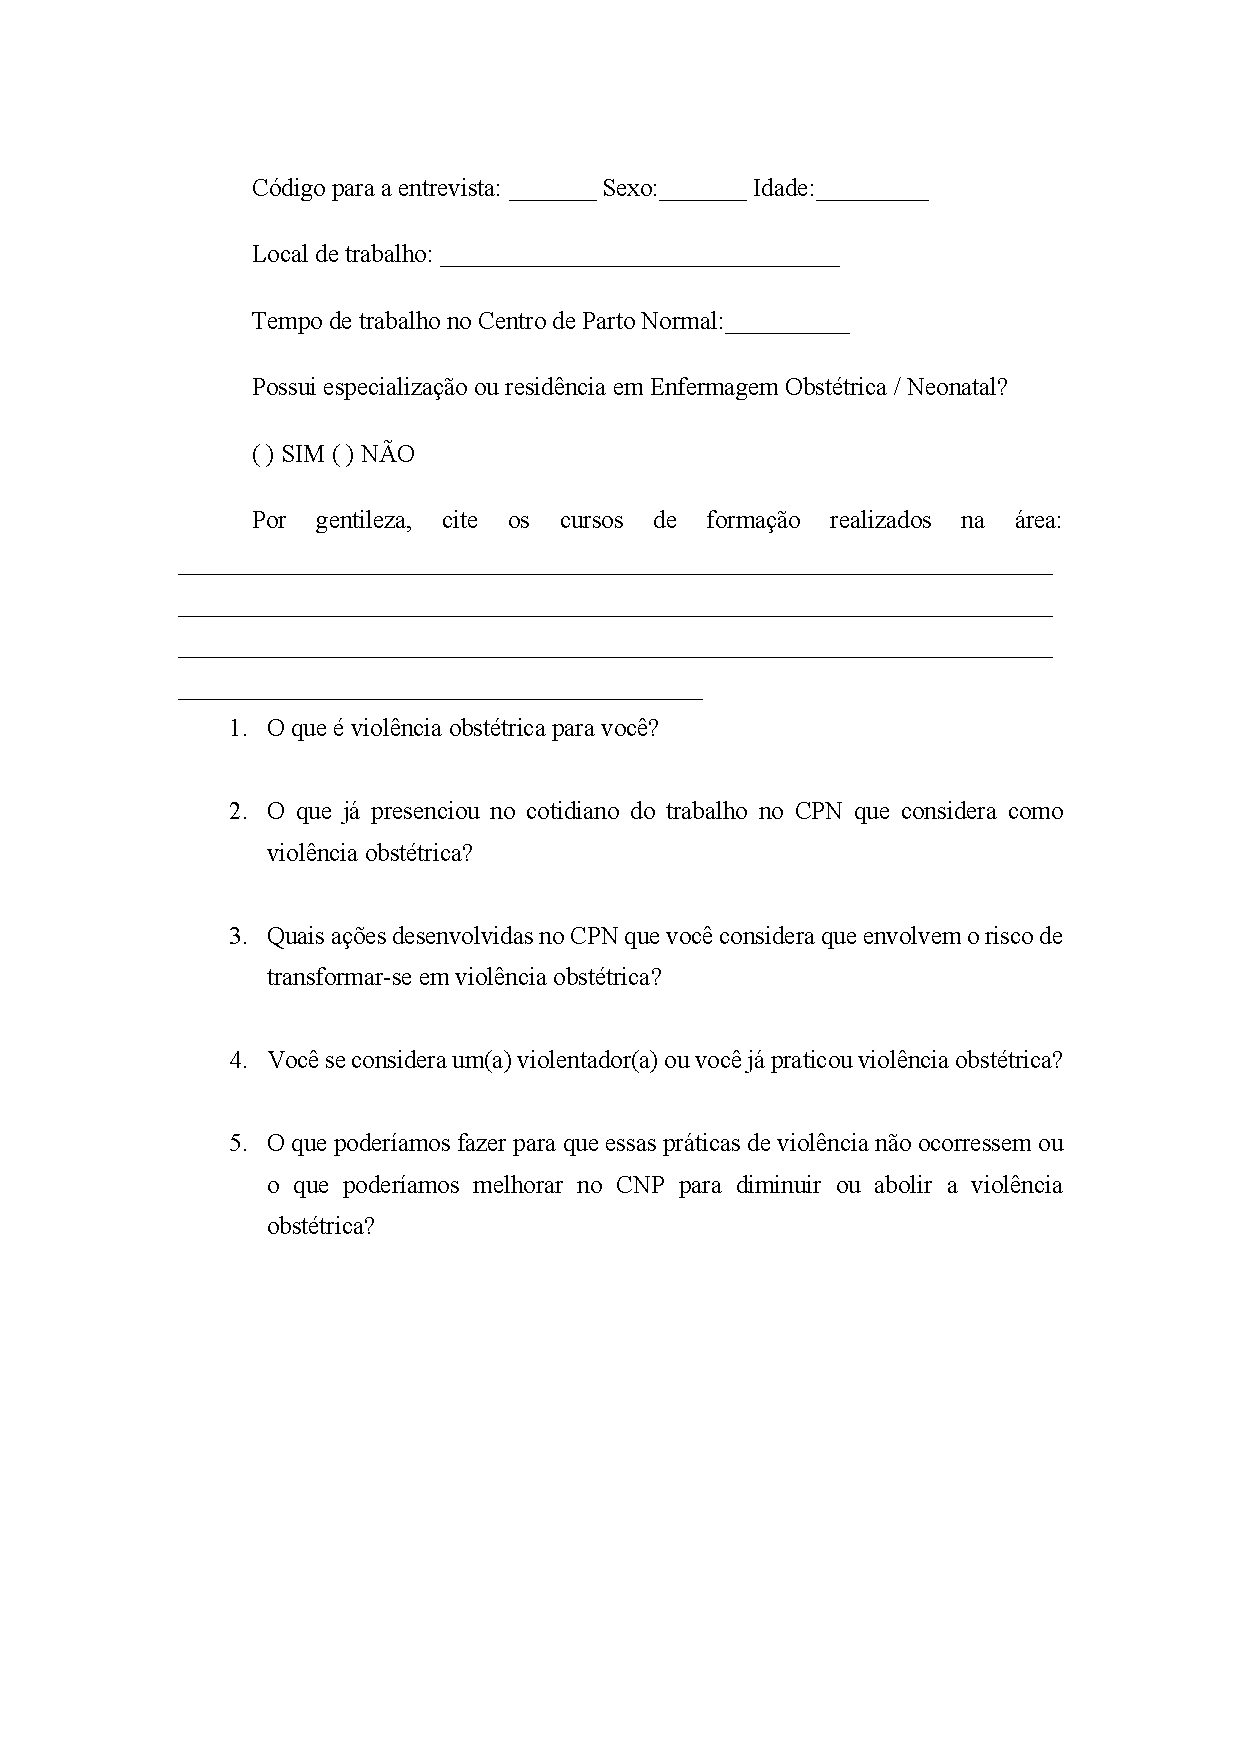
\includepdf[pages=-]{apb.pdf}
% 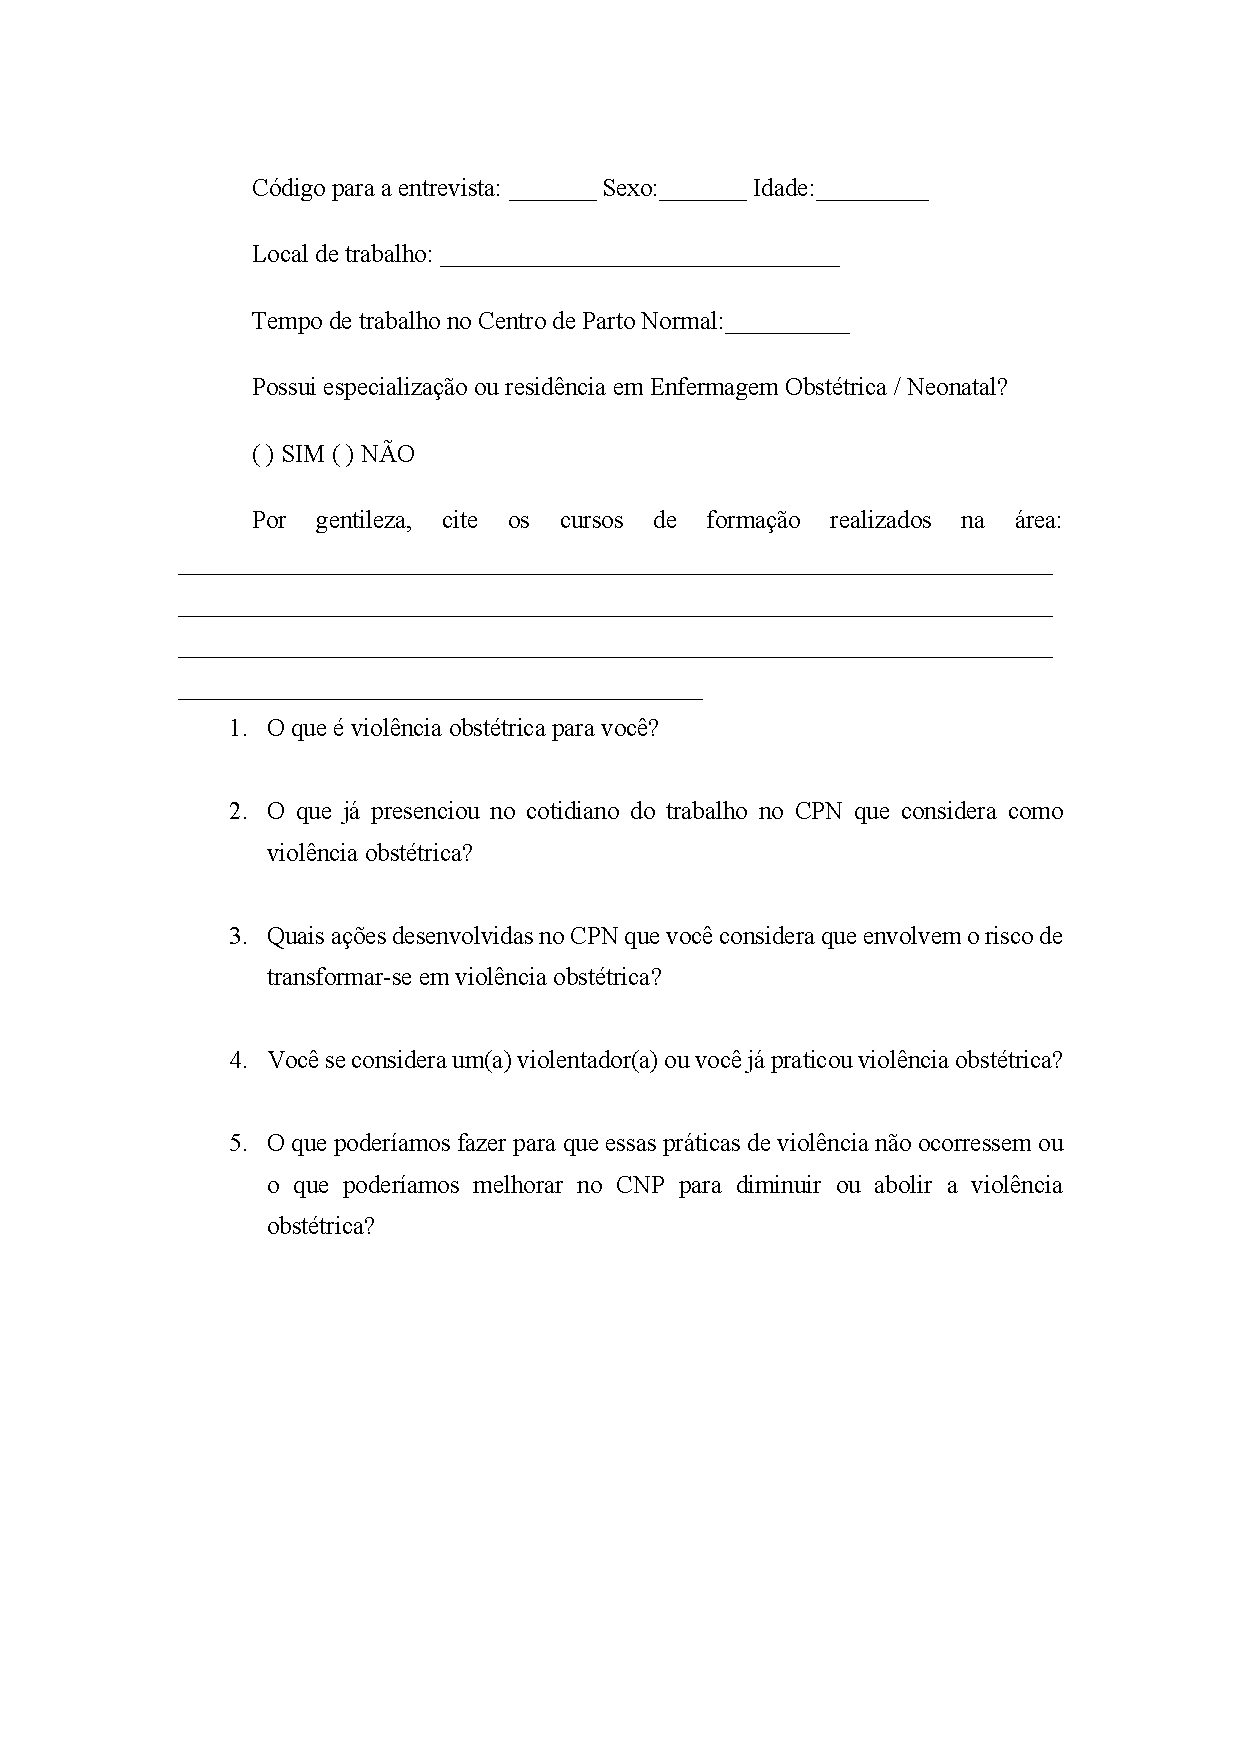
\includegraphics{apb.pdf}
\begin{figure}[htp] \centering{
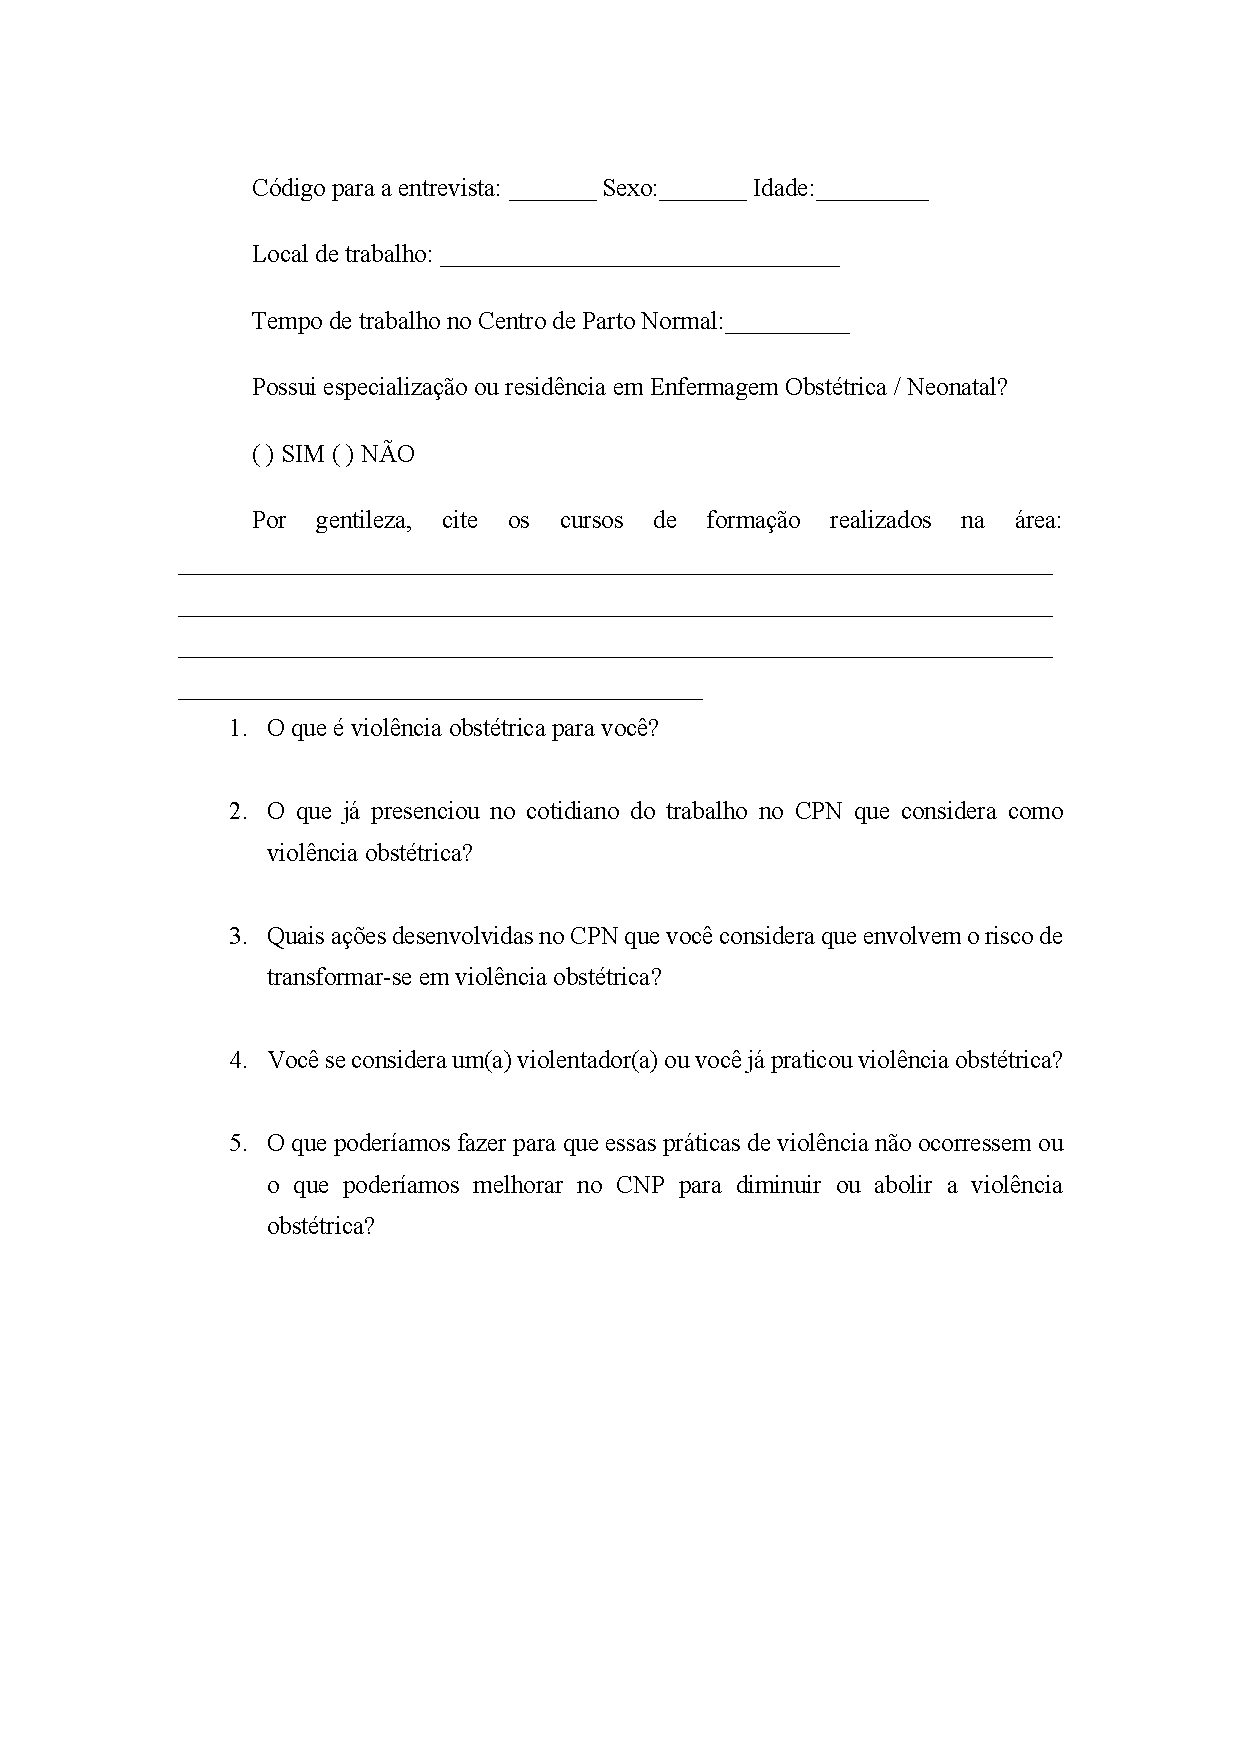
\includegraphics[scale=1]{apb.pdf}}
% \caption{Experiment 2}
\end{figure}
 
	\imprimiranexos
		% Adicione aqui os anexos do seu trabalho
		\anexo{PARECER CONSUBSTANCIADO DO CEP}
\label{an:parecer}

\includepdf[pages=-]{anexo1.pdf}

		%\anexo{Orçamento}
\label{an:orcamento}

\definecolor{midgray}{gray}{.5}

% Please add the following required packages to your document preamble:
% \usepackage{graphicx}
\begin{table}[h]
%\resizebox{\textwidth}{!}{%
\begin{tabular}{|c|c|r|r|}
\hline
OBJETOS                                                           & QUANTIDADE         & \multicolumn{1}{c|}{\begin{tabular}[c]{@{}c@{}}VALOR\\ 			UNITÁRIO\end{tabular}} & \multicolumn{1}{c|}{\begin{tabular}[c]{@{}c@{}}VALOR\\ 			TOTAL\end{tabular}} \\ \hline
\begin{tabular}[c]{@{}c@{}}Caneta\\ 			esferográfica\end{tabular} & 2                  & \begin{tabular}[c]{@{}r@{}}R\$\\ 			2,00\end{tabular}                            & \begin{tabular}[c]{@{}r@{}}R\$\\ 			4,00\end{tabular}                         \\ \hline
Fotocópias                                                        & 300                & \begin{tabular}[c]{@{}r@{}}R\$\\ 			0,10\end{tabular}                            & \begin{tabular}[c]{@{}r@{}}R\$\\ 			30,00\end{tabular}                        \\ \hline
\begin{tabular}[c]{@{}c@{}}Cartucho\\ 			de tinta\end{tabular}    & 1                  & \begin{tabular}[c]{@{}r@{}}R\$\\ 			120,00\end{tabular}                          & \begin{tabular}[c]{@{}r@{}}R\$\\ 			120,00\end{tabular}                       \\ \hline
\begin{tabular}[c]{@{}c@{}}Resma\\ 			de papel A4\end{tabular}    & 1                  & \begin{tabular}[c]{@{}r@{}}R\$\\ 			15,00\end{tabular}                           & \begin{tabular}[c]{@{}r@{}}R\$\\ 			15,00\end{tabular}                        \\ \hline
Encadernações                                                     & 3                  & \begin{tabular}[c]{@{}r@{}}R\$\\ 			10,00\end{tabular}                           & \begin{tabular}[c]{@{}r@{}}R\$\\ 			30,00\end{tabular}                        \\ \hline
Outros                                                            &                    & \multicolumn{1}{c|}{}                                                            & \multicolumn{1}{c|}{}                                                         \\ \hline
TOTAL                                                             & 307 & \multicolumn{1}{c|}{-------------}                                               & \multicolumn{1}{c|}{R\$ 199,00}                                                         \\ \hline
\end{tabular}
%}
\end{table}
	\imprimirindice

\end{document}
